Consider the following feedback system with internal delay of $T_{d}$ seconds\\
\begin{center}
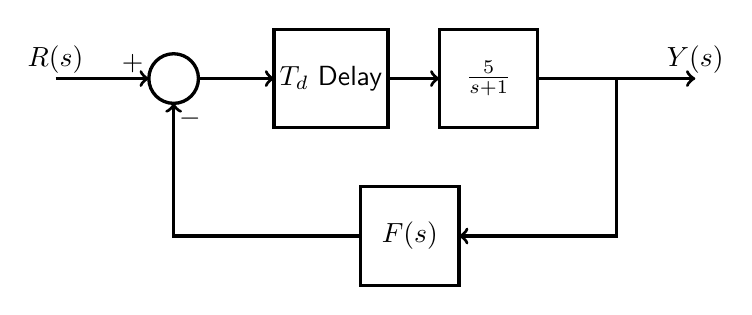
\begin{tikzpicture}[scale=1,inner sep=0pt,outer sep=0pt,very thick,
sysblock/.style={draw,rectangle,inner sep=2pt,minimum width=1.25cm,minimum height=1.25cm,very thick}]
\draw (2,0) node[draw,circle] (sum1) {$\rule{0pt}{18pt}$};
\draw (6,0) node[sysblock] (G) {$\frac{5}{s+1}$};
\draw (4,0) node[sysblock] (D) {$T_{d}$ \textsf{Delay}};
\draw (5,-2) node[sysblock] (F) {$F(s)$};

\draw[->] (.5,0) node[above=2pt] {$R(s)$} -- (sum1.180) node[above left=2pt] {$+$};
\draw[->] (sum1.0)  -- (D);
\draw[->] (D) -- (G);
\draw[->] (G.0) -- ++(2,0) node[above=2pt] {$Y(s)$};
\draw[->] (G.0) ++(1,0) |- (F);
\draw[->] (F) -| (sum1.-90) node[below right=2pt] {$-$};
\end{tikzpicture}
\end{center}
You are considering using a filter $F(s)$ to reduce sensor noise. Using the following two axes, sketch the Bode plot of the loop gain without delay for $F(s)=1$ and $F(s) = \frac{1}{s+1}$ (i.e. multiply $\frac{5}{s+1}$ by $F(s)$ in each case). Using your sketches, determine the maximum delay that can be tolerated before the closed loop system becomes unstable. You must indicate the key frequencies and calculations necessary to determine the results.\\
\includegraphics[width=3.5in]{\mainfolder/LectureNotes/\lecturefolder/HomeworkProblems/Problem09/blankbode}\includegraphics[width=3.5in]{\mainfolder/LectureNotes/\lecturefolder/HomeworkProblems/Problem09/blankbode}

